%%%% ijcai22.tex

\typeout{IJCAI--22 Instructions for Authors}

% These are the instructions for authors for IJCAI-22.

\documentclass{article}
\pdfpagewidth=8.5in
\pdfpageheight=11in
% The file ijcai22.sty is NOT the same as previous years'
\usepackage{ijcai22}

% Use the postscript times font!
\usepackage{times}
\usepackage{soul}
\usepackage{url}
\usepackage[hidelinks]{hyperref}
\usepackage[utf8]{inputenc}
\usepackage[small]{caption}
\usepackage{graphicx}
\usepackage{amsmath}
\usepackage{amsthm}
\usepackage{adjustbox}
\usepackage{booktabs}
% \usepackage{algorithm}
\usepackage{algorithmic}
\usepackage[english]{babel}
\urlstyle{same}
\usepackage{natbib}
\usepackage{xspace}
% the following package is optional:
\usepackage{latexsym}
\usepackage{xcolor}
\newcommand{\mike}[1]{\textcolor{red}{#1}}
% See https://www.overleaf.com/learn/latex/theorems_and_proofs
% for a nice explanation of how to define new theorems, but keep
% in mind that the amsthm package is already included in this
% template and that you must *not* alter the styling.
\newtheorem{exahttps://www.overleaf.com/project/63904fa168a9cddc37b275dd/detachermple}{Example}
\newtheorem{theorem}{Theorem}

\newcommand{\afriberta}{AfriBERTa\xspace}
\newcommand{\afroxlmr}{Afro-XLM-R\xspace}
 % and 

% Following comment is from ijcai97-submit.tex:
% The preparation of these files was supported by Schlumberger Palo Alto
% Research, AT\&T Bell Laboratories, and Morgan Kaufmann Publishers.
% Shirley Jowell, of Morgan Kaufmann Publishers, and Peter F.
% Patel-Schneider, of AT\&T Bell Laboratories collaborated on their
% preparation.

% These instructions can be modified and used in other conferences as long
% as credit to the authors and supporting agencies is retained, this notice
% is not changed, and further modification or reuse is not restricted.
% Neither Shirley Jowell nor Peter F. Patel-Schneider can be listed as
% contacts for providing assistance without their prior permission.

% To use for other conferences, change references to files and the
% conference appropriate and use other authors, contacts, publishers, and
% organizations.
% Also change the deadline and address for returning papers and the length and
% page charge instructions.
% Put where the files are available in the appropriate places.


\addto\extrasenglish{  
  \def\sectionautorefname{Section}  
}
\addto\extrasenglish{  
  \def\subsectionautorefname{Section}  
}
\addto\extrasenglish{  
  \def\subsubsectionautorefname{Section}  
}

% PDF Info Is REQUIRED.
% Please **do not** include Title and Author information
\pdfinfo{
/TemplateVersion (IJCAI.2022.0)
}

% \title{Fool Me If You Can: Data Corruption Impact on Named Entity Recognition for Low Resourced Languages}
\title{The Impact of Data Corruption on Named Entity Recognition for Low Resourced Languages}

% Single author syntax


% Multiple author syntax (remove the single-author syntax above and the \iffalse ... \fi here)
\iffalse
\author{
First Author$^1$
\and
Second Author$^2$\and
Third Author$^{2,3}$\And    
Fourth Author$^4$
\affiliations
$^1$First Affiliation\\
$^2$Second Affiliation\\
$^3$Third Affiliation\\
$^4$Fourth Affiliation
\emails
\{first, second\}@example.com,
third@other.example.com,
fourth@example.com
}
\fi

\begin{document}

\maketitle

\begin{abstract}
Data is often a massively limiting factor in natural language processing for low-resourced languages. In particular, there is significantly less data than for higher-resourced languages. This data is also often of low-quality, rife with errors and invalid text. Many prior works focus on dealing with these problems, either by generating synthetic data, or filtering out low-quality parts thereof. We instead investigate these factors more deeply, by systematically measuring the effect of data quantity and quality on the performance of pre-trained language models. Our results show that having a missing annotation is preferred compared to having an incorrect one; and that models can perform remarkably well with only 10\% of the training data. Finally, all of our results are very consistent across 11 languages and 4 different pre-trained models.

%%Data is often a massively limiting factor in natural language processing for low-resourced languages. In particular, there is significantly fewer data than for higher-resourced languages, and this data is often of low quality, rife with errors and incorrect annotations. Many prior works focus on dealing with these problems by generating synthetic data or filtering out low-quality parts. Instead, we investigate these problems more deeply by systematically measuring the effect of data quantity and quality on the performance of pre-trained language models on a Named Entity Recognition (NER) task. Our results show that data with missing annotations is preferable to incorrect ones and that these pre-trained models can perform remarkably well with relatively small datasets compared to those published. Finally, these results are consistent across 11 low-resourced language corpus.%%
\end{abstract}

\section{Introduction}
Natural Language Processing (NLP) is an impactful field, and has received much interest recently, and has been applied in numerous settings~\citep{vaswani2017Attention,conneau2019Unsupervised}.
However, much of the focus is on high-resourced languages~\citep{vaswani2017Attention,conneau2019Unsupervised,radford2018Improving,radford2019language_gpt2}, such as English, German, Spanish, etc. While this has led to impressive results for these languages, lower-resourced languages have often not enjoyed as much attention, leading to a large gap in NLP system performance between high- and low-resourced languages. This gap has resulted in an increasingly large body of work focused exclusively on low-resourced languages, either developing models~\citep{ogueji2021Small,alabi2022Multilingual} or introducing datasets~\citep{oyewusi2021Naijaner,adelani2021MasakhaNER,adelani2022Thousand,adelani2022Masakhaner}.

%% Natural Language Processing (NLP) has received much interest recently~\citep{vaswani2017Attention,conneau2019Unsupervised}. However, much of the focus is on high-resourced languages~\citep{vaswani2017Attention,conneau2019Unsupervised,radford2018Improving,radford2019language_gpt2}. While this has led to impressive results for these languages, low-resource language datasets are often created through less mature pipelines and do not benefit from the same amount of expertise in their acquisition, cleaning and labelling as their high-resourced counterpart. This gap has resulted in an increasingly large body of work focused exclusively on low-resourced languages through performance analysis of different NLP models on these languages~\citep{ogueji2021Small,alabi2022Multilingual} or the introduction of new datasets~\citep{oyewusi2021Naijaner,adelani2021MasakhaNER,adelani2022Thousand,adelani2022Masakhaner}.

Despite this recent work and impressive progress, data is still one large limiting factor for low-resourced NLP~\citep{adelani2022Thousand,adelani2022Masakhaner}. In particular, the two main problems are quality and quantity of data. First of all, the amount of data available for low-resourced languages is often a fraction of the high-resourced languages; and for many languages, no data exists at all. Secondly, the data that is available often has questionable quality, containing corruption, invalid tokens or just gibberish~\citep{kreutzer2021Quality}, which has detrimental downstream effects on the models trained using this data~\citep{abdul2012Extrinsic,alabi2019Massive}.

%%Despite this impressive progress, data remains a limiting factor for low-resourced NLP~\citep{adelani2022Thousand,adelani2022Masakhaner}. In particular, the two main problems are the quality and quantity of data. First of all, the amount of data available for low-resourced languages is often a fraction of the high-resourced languages; and datasets are not even available for some languages. Secondly, the available datasets are often of questionable quality, with invalid annotations or just gibberish~\citep{kreutzer2021Quality}, which has detrimental downstream effects on the models trained on these datasets~\citep{abdul2012Extrinsic,alabi2019Massive}.



The large amounts of poor-quality data has led to many works focusing on filtering data~\citep{axelrod2011Domain,xu2019Improving,imankulova2017Improving,abdulmumin-hybrid-2021,abdulmumin2022Separating} to improve results by discarding all of the invalid or corrupt portions of a dataset. In many of these works, the perspective is that there is an existing, but noisy, dataset, and it must be filtered, keeping only the high-quality parts thereof. The data quality is often so poor that having a smaller high-quality dataset can be better than having a much larger, and lower-quality, dataset. The lack of data has also spurred research into synthetically generating more data, by using techniques such as backtranslation~\citep{bojar2011Improving,lambert2011Investigations,sennrich2015Improving} or using a translation model to generate labelled data for one language using by translating another language's dataset.

% An additional field of research aims to synthetically generate more data
%%The large amounts of poor-quality data have led to many works focusing on filtering data~\citep{axelrod2011Domain,xu2019Improving,imankulova2017Improving,abdulmumin-hybrid-2021,abdulmumin2022Separating} to improve results by discarding all of the invalid or corrupt portions of a dataset. In many of these works, the perspective is that data is available but noisy and must be cleaned, keeping only the high-quality parts. In some cases, the quality of some datastes is often so poor that having a smaller high-quality dataset can be better than having a larger but low quality dataset. (TODO: cite this)

% The lack of data has also spurred research into synthetically generating more data, by using techniques such as backtranslation~\citep{bojar2011Improving,lambert2011Investigations,sennrich2015Improving} or using a translation model to generate labelled data for one language using by translating another language's dataset. Yet other works acknowledge that limited data is given, and attempt to leverage transfer learning~\citep{madx,adelani2021MasakhaNER,adelani2022Masakhaner,alabi2022Multilingual} from other languages that have datasets to improve performance on the target language.


We instead take a different perspective, and focus on analysing the effect of systematically reducing the quality of datasets, and examine the implications of this. In particular, we focus on a Named-Entity Recognition (NER) task due to its prevalence in many NLP systems and the existence of a few high-quality datasets in low-resourced languages. We further focus on fine-tuning existing pre-trained language models, as this is a common and high-performing approach, especially for low-resourced languages~\citep{ogueji2021Small,adelani2021MasakhaNER,alabi2022Multilingual}. We specifically focus on corrupting the training datasets in specific ways to examine the effects of data quality on the performance of models. We further alter the amount of data that the models train on to investigate the effect of the amount of training data on performance.

%% Instead, we choose to look at this problem from a different perspective by analysing the effect of systematically reducing the quality of datasets on NLP models. In particular, we focus on a Named-Entity Recognition (NER) task due to its prevalence in many NLP systems and the error-prone nature of its annotation pipeline due to the requirement of providing annotations at a word level. We further focus on fine-tuning existing pre-trained language models, as this is a common and high-performing approach, especially for low-resourced languages~\citep{ogueji2021Small,adelani2021MasakhaNER,alabi2022Multilingual}. We specifically focus on corrupting the training datasets in specific ways to examine the effects of data quality on the performance of these NER models. We further alter the amount of data used to train our models and investigate the impact on their performance.

Our results reveal an interesting  phenomenon, where the performance dropoff is not linear, i.e. training on 10\% of the data does not result in 10\% of the performance of training on the entire dataset, but rather close to 80\%. We further find that having a wrong label in NER is more damaging than having a missing label -- suggesting that when annotators are uncertain, leaving out an annotation is preferable compared to having a wrong one. Finally, we note that our results are consistent across 11 languages and 4 pre-trained models, suggesting that these observations are generally valid.

%Our results reveal an interesting phenomenon where the performance variation is not linear when altering data quantity, i.e. a linear improvement in data quantity does not produce a linear improvement in our models' performance. We further find that wrong labels in NER are more detrimental than missing ones, suggesting that when annotators are uncertain, leaving out an annotation is preferable to having a wrong one. Finally, we note a consistency in our results across 11 languages and four pre-trained models, suggesting that these observations are generally valid.

\section{Background and Related Work}
\subsection{Named Entity Recognition}
Named entity recognition (NER) is a token classification task, where the task is to classify each token in a text as an Organisation, Location, Person, Date, or ``Other''. NER as a field has many impactful applications~\citep{sang2003introduction_conll,lample2016Playing}.

A typical NER dataset consists of multiple sentences, with each sentence containing both the words and their associated labels.
The prevailing approach to train NER models is to use a pre-trained large language model (such as BERT~\citep{devlin2019BERT}, XLM-Roberta~\citep{conneau2019Unsupervised}, etc.) and fine-tune it on a small amount of NER data~\citep{conneau2019Unsupervised,adelani2021MasakhaNER}.

% \mike{What do we want to say here?}
\subsection{Data Collection and Annotation}
Since the lack of data has traditionally been a major limiting factor for low-resourced NLP research, multiple different approaches have developed to effectively collect data in resource-constrained settings. In particular, community involvement has played a large part in this~\citep{nekoto2020Participatory,nekoto2022Participatory}, where native speakers annotate or create datasets to be used in research. This has led to the creation of many different datasets~\citep{adelani2021MasakhaNER,nekoto2022Participatory}, but it relies on community members instead of trained annotators, which may result in some aspects of the annotation being less accurate. Furthermore, while this approach can successfully develop datasets for low-resourced languages, due to logistic challenges and a limited amount of unlabelled text, these datasets are often significantly smaller than high-resourced datasets~\citep{conneau2019Unsupervised,adelani2021MasakhaNER}.
% \subsection{Data Filtering and such}

\subsection{Lack of Quality and Quantity in Low-resourced Languages}
% \cite{alabi2019Massive}
While there has been significantly progress in recent years, datasets low-resource language are often quite small and limited, or exhibit subpar quality. Both of these factors can lead to badly-performing models. 
For instance, \citet{kreutzer2021Quality} perform a large-scale audit of several web-scale and automatically extracted multilingual datasets, and find that the quality is often poor, with rubbish characters and sentences being commonplace. Other work has focused instead on the effect of quality on the performance of downstream models.

This lack of quality can have great effects. \citet{alabi2019Massive} show that for certain low-resourced African languages, using a significantly smaller, but curated dataset outperforms training a model on a large, but noisy dataset. \citet{abdulmumin2022Separating} find similar results, where training on filtered data of higher quality improved the performance of translation models for low-resourced languages.

These two observations; that data is often of low-quality and that a smaller, higher-quality dataset is often preferred has led to much work being done on filtering existing datasets, to extract a smaller, but higher-quality subset of sentences. For instance, \citet{abdulmumin2022Separating} filter a large, automatically-aligned dataset, and find that this improved the performance of translation models for low-resourced languages.

The second factor that can limit progress in NLP is a lack of datasets for many languages, or much smaller datasets for low-resourced languages compared to higher-resourced ones~\citep{adelani2022Thousand}.




% \mike{TODO we do not speak about quantity here}

% In the case of low-resourced languages, the quality of data is often subpar, which can lead to poor results for models trained on it. For instance, \citet{kreutzer2021Quality} perform a large-scale audit of several web-scale and automatically extracted multilingual datasets, and find that the quality is often poor, with rubbish characters and sentences being commonplace. Other work has focused instead on the effect of quality on the performance of downstream models. \citet{alabi2019Massive} show that for certain low-resourced African languages, using a significantly smaller, but curated dataset outperforms training a model on a large, but noisy dataset. \citet{abdulmumin2022Separating} find similar results, where training on filtered data of higher quality improved the performance of translation models for low-resourced languages.

\section{Methodology}
% \textbf{Can we have a figure that illustrates each of these. E.g. I am thinking a bunch of sentences and then showing the effect of each corruption strategy to just make it more clear.}
\label{sec:method}
Our aim is to analyse and quantify the impact of data corruption on the performance of pre-trained language models. It would allow us to better reason about the importance of quality and quantity of data, ideally informing the future data creation processes for low-resourced languages.

While we can corrupt NER text corpora in various ways, we choose corruptions that simulate a mislabelling scenario during the annotation process, e.g. mislabelling a person in a sentence as an organisation. There are two main reasons for this choice. Firstly, many NER datasets are formed by taking an existing text source, which is usually of high quality, such as news data~\citep{adelani2021MasakhaNER} and annotating each word; thus, errors are more likely to crop up during the annotation process. Secondly, it is challenging to corrupt the base sentences in a reasonable, quantifiable and incremental way, as sentences encompass meaning which is often hard to change atomically.

Thus, we focus on corrupting only the labels, using different strategies detailed in \autoref{sec:corrupt_strats}. For each corruption strategy, we uniformly vary the amount of corruption and train our models using the new, corrupted dataset. This process allows us to evaluate how each corruption strategy affects the model as we vary the degree of corruption. We discussed the data for this study in \autoref{sec:data}.
 
% The reason for this choice was influenced by the knowledge of the infrastructure that surrounds the collection of data in low-resource scenarios. \textbf{TODO: elaborate here a bit more, i.e. what infrastructure?} Therefore, when designing corrupt strategies, we focus on the labels attached to the sentences but not the sentences themselves. Another reason is that it would be much more difficult to quantifiably corrupt the sentences in the datasets as sentences encompass meaning which is often hard to change incrementally. For each corruption strategy, described in the next section, we vary the amount of corruption and train our models on each setting. This allows us to evaluate how much each corruption strategy affects the model, with various degrees of corruption.
% \textbf{TODO: TALK ABOUT THE RANGE AND STUFFS}

\begin{figure*}
    \centering
    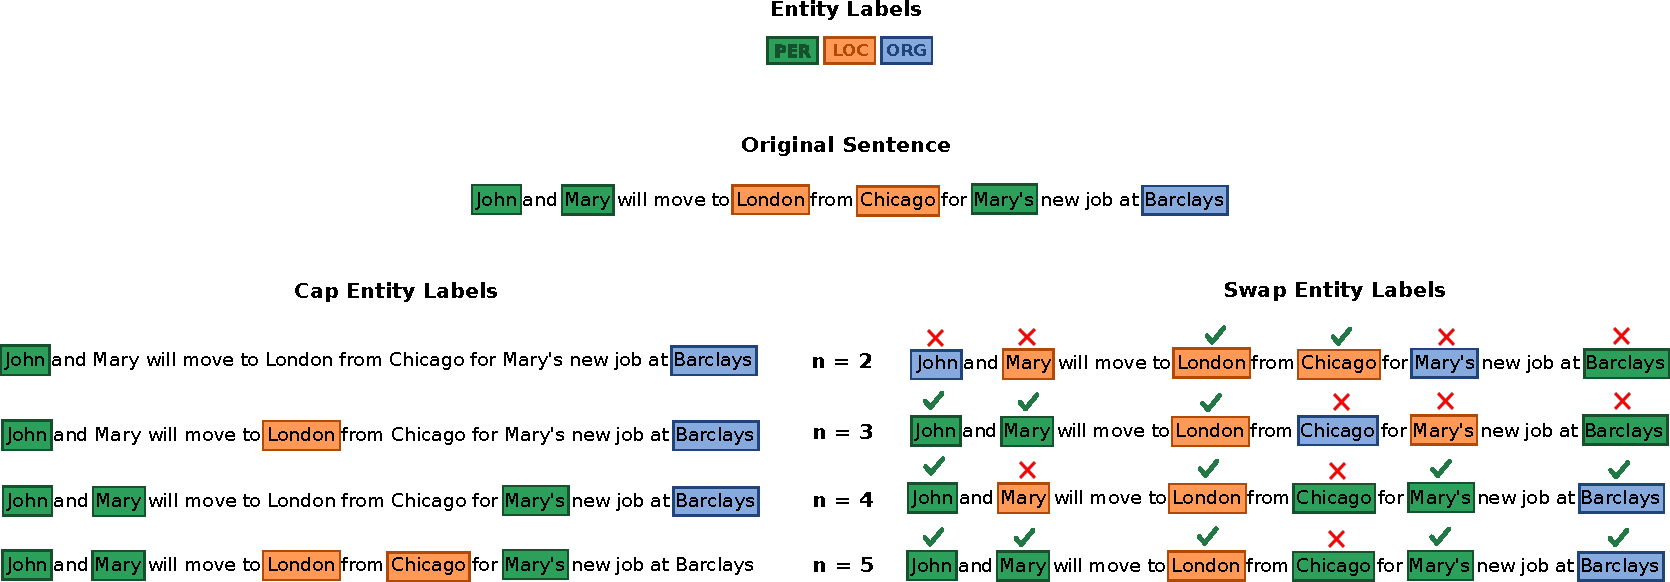
\includegraphics[width=1\linewidth]{images/diagram.pdf}
    \caption{An illustration of the different corruption strategies we use. (Left) When capping labels, we effectively remove a certain number of labels, replacing them with ``O''. (Right) When swapping labels, we instead randomly replace a label with an incorrect one. In these figures we illustrate the \textit{local} version of the corruptions, with $n$ being the parameter that determines the number of labels kept unchanged.}
    \label{fig:main_fig}
\end{figure*}


\subsection{Different Corruption Strategies}
\label{sec:corrupt_strats}
We describe the corruption strategies in the next sections, and \autoref{fig:main_fig} shows some examples of the different strategies we consider. For corruption strategies involving the quality of labels, we consider the atomic element to be a single NER entity label, even if this consists of multiple words. Thus, when we change the label of a specific entity, we always change its span instead of just a part thereof. Also, we only change the train data while leaving the evaluation data unchanged. The reason for this is because we want an objective comparison of different corruption strategies. A visual illustration of our quality-related corruption strategies can be found in \autoref{fig:main_fig}.
% \mike{TODO say we do an entire entity instead of randomly swapping things on a per word basis. Also say test dataset is the same, unmodified}
\subsubsection{Sentence Pruning}
\label{sec:method:pruning}

Dataset annotation is generally an expensive and logistically challenging process (\mike{ToDo cite this}) when more than one participants are involved. As a result, low-resourced NLP datasets are often not particularly big. Due to this observation, we first evaluate the effect of varying the amount of data available to the models. In this strategy, we randomly remove sentences from the original dataset to create sub-datasets with fewer sentences than the original dataset. This process allows us to measure the model performance as a function of data quantity. We choose to represent quantity as a function of the number of sentences because removing words can alter the meaning impacting the model performance in ways we can't control.

% The strategy simulates a simple scenario where the quantity of data at a sentence level is of low quantity. Taking a step back to look at how NER works, we usually train our models with corpora made up of sequence pairs. Each sequence represents a sentence and its annotations (consisting of NER tokens). Therefore, in this strategy, we randomly remove sentences from the original dataset so as to create sub-datasets with different numbers of sentences all lower that the number of sentences in the original dataset. The objective is the examine the performance of our models trained with these sub-datasets compared to those trained on the original one. 

\subsubsection{Entity Label Capping}
\label{sec:method:cap}

A rich NER dataset would be a dataset that has a high annotation density, i.e. a high number of annotated entities per sentence.
% . In other words, high number of annotated entities per sentence gives the ability for a model to learn a rich set of labels.
This strategy aims at inhibiting the model by thresholding the number of entity annotations allowed in the dataset. In the real world, this would be equivalent to a situation where an annotator failed to label a particular span of token as one of entities PER, LOC, ORG, DATE, instead giving it the default entity type O, which generally means \textit{not relevant}.

We have two variations of this corruption, \textit{local} and \textit{global}. Local means that we have a per-sentence threshold for the number of annotations; for instance, if this threshold is $2$, we keep only $2$ annotations per sentence, deleting (i.e. setting to O) the others. Global, on the other hand, means that we keep only a certain percentage of labels across the entire dataset; for example, $50\%$ would mean that we randomly remove half of all the labels. This, in contrast to the local setting, may leave some sentences unmodified, or completely remove all annotations from certain sentences.

% We perform this corruption at a global and local level. Here global means that we set a threshold for an entire corpus while local means that this threshold is set per sentence. Therefore a local label capping will threshold the number of entities allowed per sentence while a global one will threshold the amount for the entire corpus irrespective sentence where the entity removed came from.

\subsubsection{Entity Label Swapping}
\label{sec:method:swapping}

Another scenario that could happen during the annotation procedure would be the mislabelling of a span of tokens with the wrong entity. For example, the organisation \textit{John Deere} is mistakenly labelled as a person. This creates a situation where there are contradictory labels, with the same token potentially having different labels, some correct and some incorrect. The goal behind this strategy is to determine how robust large pre-trained language models are to such contradictions. 
In the same spirit as the previous corruption strategies, we corrupt the datasets at a local and global level by either setting a threshold per sentence or across the entire corpus.


%setting threshold of label allowed to be un-corrupted at a sentence and corpus level.
% This indeed, creates a situation where the labels contradicts themselves by have  different tokens having very similar word contexts but with different labels. The objective here is to see how robust large pre-trained language model are to such scenarios. Recall that we only change the labels but not the sentences themselves. Also, in the same spirit as the previous corruption strategies, we try to evaluate this at a local and global level by setting threshold of label allowed to be un-corrupted at a sentence and corpus level.
\subsection{Data}
\label{sec:data}
We use the MasakhaNER dataset~\citep{adelani2021MasakhaNER}, which is a high-quality dataset for 10 low-resourced, African languages. We specifically focus on low-resourced languages, as these languages often suffer from the aforementioned quality and quantity problems. Furthermore, this dataset is of high-quality, which allows us to evaluate the full spectrum of quality, from gold-standard to completely corrupted. Additionally, we have 10 different languages to evaluate how much the specific language affects the results.

Finally, as a baseline, we also use the CONLL NER dataset, which is a staple NER dataset in English~\citep{sang2003introduction_conll}.

\autoref{tab:num_sentences} contains information about the relative sizes of each language's dataset and \autoref{fig:barchart_num_ents} shows how many entities of each type there are per language.

% \mike{TODO elaborate more and maybe say sentence numbers, etc.}

% \mike{Justify more why we use low resourced languages}
% We describe the different strategies we use in the next sections.

\begin{table}[]
    \centering
    \caption{The number of sentences for each NER dataset we consider.}
    \label{tab:num_sentences}
    \begin{adjustbox}{width=1\linewidth}
    \begin{tabular}{lr}
\toprule
     Language &  Number of Sentences \\
\midrule
          hau &                 1912 \\
          pcm &                 2124 \\
          ibo &                 2235 \\
          lug &                 1428 \\
          kin &                 2116 \\
          wol &                 1871 \\
conll\_2003\_en &                14042 \\
          luo &                  644 \\
          swa &                 2109 \\
          amh &                 1750 \\
          yor &                 2171 \\
\bottomrule
\end{tabular}

    \end{adjustbox}
\end{table}

\begin{figure}
    \centering
    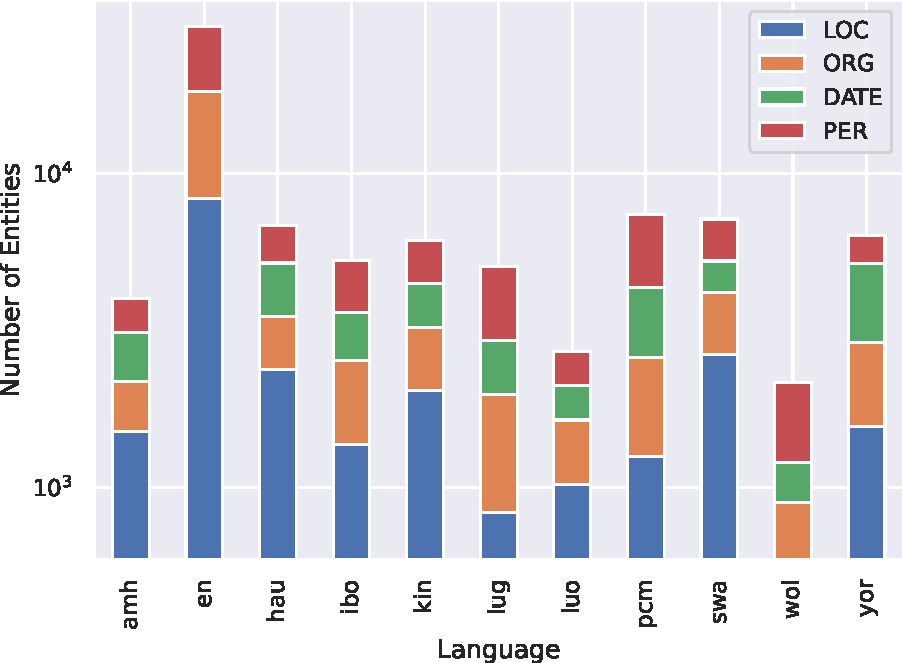
\includegraphics[width=1\linewidth]{images/number_entities.pdf}
    \caption{Number of Entities per Language}
    \label{fig:barchart_num_ents}
\end{figure}

\subsection{Metrics}
In addition to considering the overall classification F1 score for each model, we consider the uncertainty of the models as the level of data corruption increases. This allows us quantify the effect of corruption on the certainty and confidence of the models. In particular, we use the \textit{entropy} \textbf{TODO}.

\section{Experiments}
Having described our corruption strategies, we now perform our experiments and showcase our results. We consider the five corruption strategies described above, and use 4 different pre-trained language models, described in \autoref{sec:diff_models}. Each run consists of fine-tuning a single pre-trained model on a single language's dataset, either the original one or a corrupted version.
We run all experiments over 3 seeds and average the results to obtain a more accurate performance estimation. The metric we use is the F1 score, as that is commonly used as the main metric when evaluating NER models~\citep{sang2003introduction_conll,adelani2021MasakhaNER}.
We specifically investigate the effect of progressively corrupting data on the performance of each model. This simulates the effect of having subpar data quality (for instance due to incorrect annotations), but allows us to study this in a controlled setting. We do not modify the test datasets at all.

Then, to normalise results across languages, we divide each F1 score by the value obtained when training with the full, uncorrupted dataset. This effectively measures what fraction of performance is lost and allows us to transform all of the metrics to fall between 0 and 1, resulting in the results being comparable across languages and models. We then average all of our results over the 11 languages and plot the mean and standard deviation. We first examine the effect of quantity in \autoref{sec:exp_quantity} and then move to understanding the implications of data quality in \autoref{sec:exp_quality}.

\subsection{Different Pre-trained Language Models}
\label{sec:diff_models}
We use four different pre-trained language models. We first consider two models developed specifically for low-resourced African languages, \afriberta and \afroxlmr. \afriberta~\citep{ogueji2021Small} was pre-trained on less than 1GB of African language text. \afroxlmr~\citep{alabi2022Multilingual} used \textit{language adaptive fine-tuning}, where a pre-trained language model is fine-tuned on unlabelled data using the same objective as was used during pre-training. \afroxlmr performed this process on 20 languages, 17 of them from Africa, starting from XLM Roberta. XLM Roberta~\citep{conneau2019Unsupervised} is a high-performing model that was pre-trained on 100 languages. Finally, Multilingual BERT~\citep{devlin2019BERT} used the standard BERT training process on 104 languages using data from Wikipedia.

We have two models pre-trained or adaptively fine-tuned on low-resourced, African languages, some of which are contained in our dataset. The other two models are traditional multilingual models, with the majority of the training datasets consisting of high-resourced languages. All of these models have been shown to perform well in the NER task~\citep{adelani2021MasakhaNER,ogueji2021Small,alabi2022Multilingual}. We choose the specific model versions to be roughly comparable in terms of number of parameters. More information about the models is included in \autoref{tab:plms}.
% We use the following four pre-trained language models (TODO explain and say on which langs they were trained and number of parameters):
% \begin{description}
%     \item[AfriBerta] \texttt{afriberta-large}\footnote{\url{https://huggingface.co/castorini/afriberta_large}} \citet{ogueji2021Small}
%     \item[\afroxlmr] \texttt{afro-xlmr-base}\footnote{\url{https://huggingface.co/Davlan/afro-xlmr-base}} \citet{alabi2022Multilingual}.
%     \item[XLM Roberta] \texttt{xlm-roberta-base}\footnote{\url{https://huggingface.co/xlm-roberta-base}} \citet{conneau2019Unsupervised}
%     \item[Multilingual BERT]  \texttt{bert-base-multilingual-cased}\footnote{\url{https://huggingface.co/bert-base-multilingual-cased}} 110M params \citet{devlin2019BERT}
% \end{description}


\begin{table*}[h]
    \centering
    \caption{Information about the different pre-trained language models we use.}
    \label{tab:plms}
    \begin{adjustbox}{width=1\linewidth}
    \begin{tabular}{llllp{0.3\linewidth}}
        \toprule
        Name & Name & Source & Parameters & African Languages \\
        \midrule
        \afriberta & {\texttt{afriberta-large}} & \citet{ogueji2021Small} & 126M  & amh, hau, ibo, kin, pcm, swa, yor \\
        \afroxlmr & \texttt{afro-xlmr-base} & \citet{alabi2022Multilingual} & 270M?  & amh, hau, ibo, kin, pcm, swa, yor \\
        XLM Roberta & \texttt{xlm-roberta-base} & \citet{conneau2019Unsupervised} & 270M?  & amh, hau, swa \\
        Multilingual BERT & \texttt{bert-base-multilingual-cased} & \citet{devlin2019BERT} & 110M  & swa, yor \\
        \bottomrule
    \end{tabular}
    \end{adjustbox}
\end{table*}

\subsection{Initial Results}
In \autoref{tab:performance_all}, we show the results when training on the entire training dataset, grouped by model. Overall, most models perform well on most languages, with \afroxlmr performing the best on average. mBERT, on the other hand, performs the worst overall, and even has 0 F1 score on Amharic, as it was not pre-trained on data containing this script~\citep{adelani2021MasakhaNER}.

\subsection{Quantity}
\label{sec:exp_quantity}
Here we investigate the effect of data quantity on the performance of the models. We specifically remove a certain percentage of the data and train the model on the remaining ones. Furthermore, since the specific fraction we keep/delete may have an effect, we run this experiment three times, each time with different random selections of data. We average over these three permutations, and find that the results are very similar across them.

In \autoref{fig:global_cap_sentences}, we examine the performance when randomly removing a certain percentage of sentences from the datasets. The results here emphasise that the relationship between quantity and performance is highly non-linear.
For instance, when only having 60\% of the sentences from the original dataset, the performance is nearly the same as using 100\% of the data. Even more shockingly, when keeping only 10\% of the data, \afriberta still retains 80\% of the performance of training on the full data. Other models, such as XLMR, perform slightly worse, but still reaches roughly 70\% performance at 10\% of the data. When using even less data, such as 1\% or 5\%, we do see a sharp dropoff and much worse performance. This may be due to the phenomenon observed by \citet{mindermann2022Prioritized}, where there are many datapoints that do not add in additional information, and do not need to be relearnt.

% \textbf{Hey, what about effect of data quantity on transfer?}

% \textbf{Should we not run things here where we have multiple seeds when dropping -- to see how the exact sentences we drop affects the results?}
% \mike{TODO Cite \citet{mindermann2022Prioritized}}
\subsection{Quality}
\label{sec:exp_quality}
We now consider the effect of quality on performance, specifically looking at the different corruption strategies mentioned in \autoref{sec:method}. 
\subsection{Global}

In \autoref{fig:global_cap_labels}, we delete a specific fraction of labels, replacing them with the wrong value ``O''. Here, the performance dropoff is not quite linear, with keeping only 60\% of the labels resulting in 80\% performance. Even having only 40\% of the labels provides 60\% performance.

\autoref{fig:global_swap_labels} considers a similar scenario, but instead swaps a fraction of the labels with another incorrect entity label. Here we see a much more linear relationship, indicating that performance is more sensitive to the wrong label than a missing one.
\subsection{Local}
Now, considering the local perturbations, \autoref{fig:local_cap_labels} caps the number of labels per sentence, and replaces all excess labels with ``O''. Here we see that having two labels per sentence is sufficient to recover 80\% performance, and 4 entities is enough to obtain near full performance. In \autoref{fig:local_swap_labels}, we see a more aggressive trend, where swapping one label per sentence with an incorrect one results in 60\% performance, and swapping 2 results in an abysmal 30\%. This again emphasises that incorrect labels are far more damaging to the model's performance compared to merely removing labels.
% \textbf{Hey in the cap labels figure, capping at 1 also results in 60\% performance}

\begin{table}[]
    \centering
    \caption{The performance of each pre-trained model when fine-tuning on unaltered training data. The best performance per language is marked in bold.}
    \label{tab:performance_all}
    \begin{adjustbox}{width=1\linewidth}
    \begin{tabular}{lllllr}
\toprule
Model &            AfriBERTa &           Afro-XLM-R &       XLM-R &                mBERT & Average \\
Language &                      &                      &             &                      &         \\
\midrule
amh      &           72.1 (0.9) &  \textbf{75.9 (1.9)} &  71.9 (0.9) &            0.0 (0.0) &    55.0 \\
en       &           88.5 (0.3) &  \textbf{92.8 (0.1)} &  92.7 (0.2) &           92.6 (0.2) &    91.7 \\
hau      &           90.0 (0.5) &  \textbf{90.8 (0.4)} &  89.8 (0.2) &           87.2 (0.5) &    89.5 \\
ibo      &  \textbf{87.1 (0.3)} &           87.0 (0.6) &  83.2 (0.2) &           84.7 (0.5) &    85.5 \\
kin      &           74.1 (0.7) &  \textbf{78.1 (0.2)} &  72.5 (1.3) &           70.7 (0.5) &    73.8 \\
lug      &           78.7 (0.2) &  \textbf{81.3 (0.2)} &  77.7 (0.4) &           79.6 (0.7) &    79.3 \\
luo      &           68.1 (0.9) &           69.2 (4.9) &  69.4 (2.2) &  \textbf{71.7 (0.9)} &    69.6 \\
pcm      &           85.5 (0.6) &  \textbf{89.2 (0.3)} &  86.2 (1.5) &           88.0 (0.1) &    87.2 \\
swa      &           87.5 (0.6) &  \textbf{88.3 (0.2)} &  87.5 (0.6) &           86.0 (0.7) &    87.3 \\
wol      &           61.4 (1.4) &  \textbf{66.1 (1.6)} &  63.9 (0.8) &           63.4 (0.9) &    63.7 \\
yor      &           79.3 (0.6) &  \textbf{80.9 (1.0)} &  76.5 (1.1) &           78.7 (0.7) &    78.8 \\
\midrule
Average  &                 79.3 &                 81.8 &        79.2 &                 73.0 &    78.3 \\
\bottomrule
\end{tabular}

    \end{adjustbox}
\end{table}




\begin{figure*}
    \centering
    \begin{minipage}[t]{0.33\linewidth}
        \captionsetup{width=.8\linewidth}
        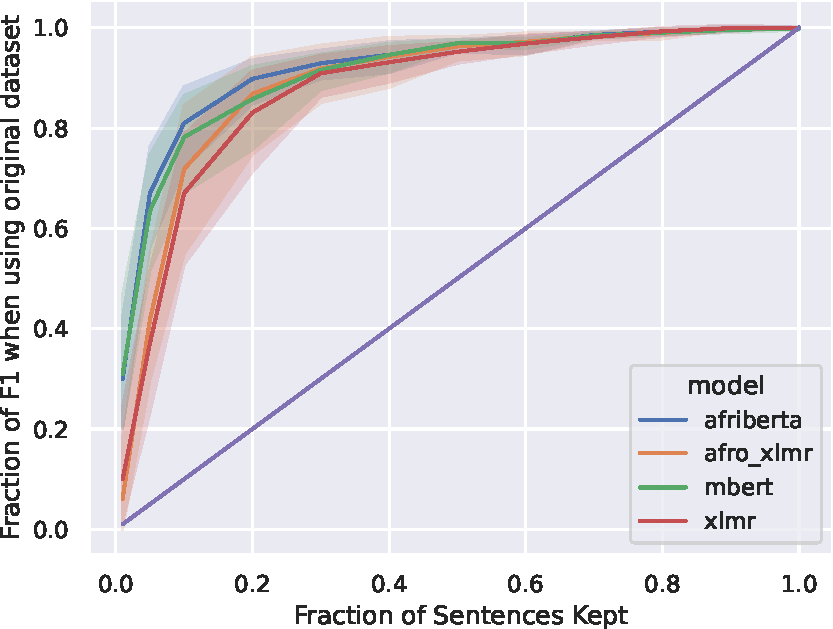
\includegraphics[width=1\linewidth]{images/global_cap_sentences.pdf}
        \caption{Showing the effect of training on a subset of data on the final performance of the models.}
        % Plotting the fraction of sentences kept against performance (measured as a fraction of ``optimal'' performance -- where the entire dataset is used). Standard Deviation across 11 languages is shaded.
        \label{fig:global_cap_sentences}
    \end{minipage}
    \begin{minipage}[t]{0.33\linewidth}
    \captionsetup{width=.8\linewidth}
        \centering
        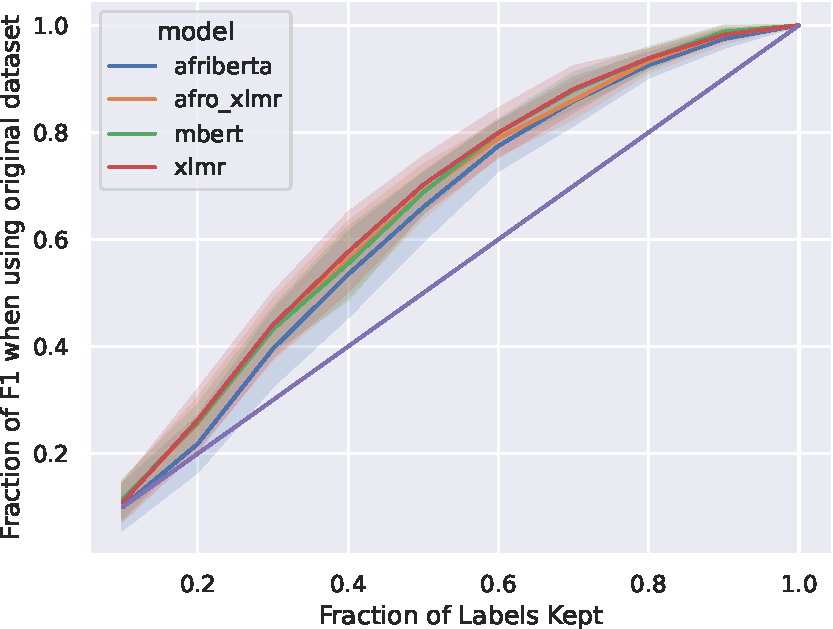
\includegraphics[width=1\linewidth]{images/global_cap_labels.pdf}
        \caption{Showing the effect of deleting a certain fraction of labels across the entire dataset, replacing them with O.}
        \label{fig:global_cap_labels}
    \end{minipage}
    \begin{minipage}[t]{0.33\linewidth}
        \captionsetup{width=.8\linewidth}
        \centering
        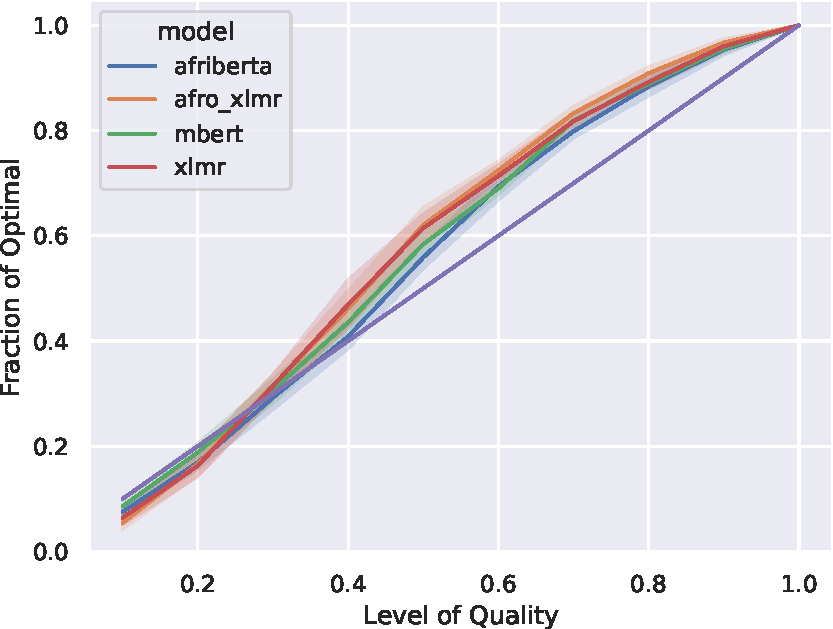
\includegraphics[width=1\linewidth]{images/global_swap_labels.pdf}
        \caption{Showing the effect of swapping a certain fraction of labels across the entire dataset, replacing the correct annotation with an incorrect entity.}
        \label{fig:global_swap_labels}
    \end{minipage}
    \caption*{Here we plot the performance (measured as a fraction of ``optimal'' performance -- where the entire dataset is used) as we change the (a) fraction of the sentences we use for training or (b) the level of corruption in a dataset. These three figures contain the \textit{global} corruptions, where we alter the entire dataset according to some corruption percentage. Standard Deviation across 11 languages is shaded.}
\end{figure*}



\begin{figure*}
    \centering
    \begin{minipage}[t]{0.45\linewidth}
        \centering
        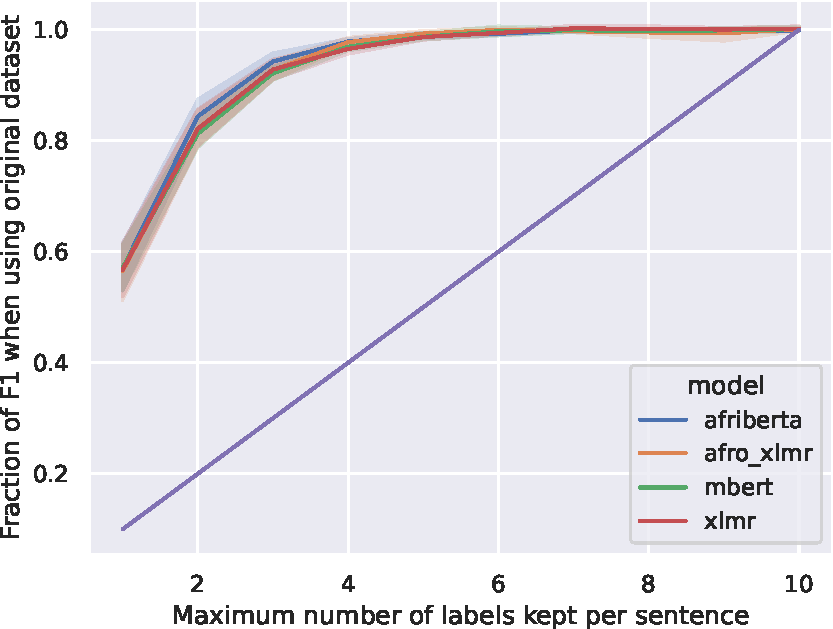
\includegraphics[width=1\linewidth]{images/local_cap_labels.pdf}
        \caption{Local Cap Labels}
        \label{fig:local_cap_labels}
    \end{minipage}
    \begin{minipage}[t]{0.45\linewidth}
    \captionsetup{width=.8\linewidth}
        \centering
        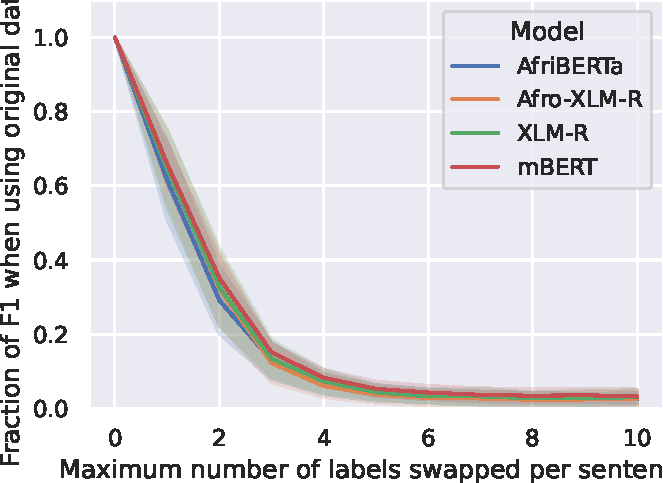
\includegraphics[width=1\linewidth]{images/local_swap_labels.pdf}
        \caption{Local Swap Labels}
        \label{fig:local_swap_labels}
    \end{minipage}

    \caption*{Here we plot the local corruptions strategies, where we either (a) cap the number of labels per sentence, replacing the excess ones with O; or (b) swap a certain number of labels per sentence with an incorrect entity. Standard Deviation across 11 languages is shaded.}
\end{figure*}

% \begin{figure}

% \end{figure}

% \begin{figure}

% \end{figure}



% \begin{figure}

% \end{figure}

% \begin{figure}

% \end{figure}
% % --

% \begin{figure}
%     \centering
%     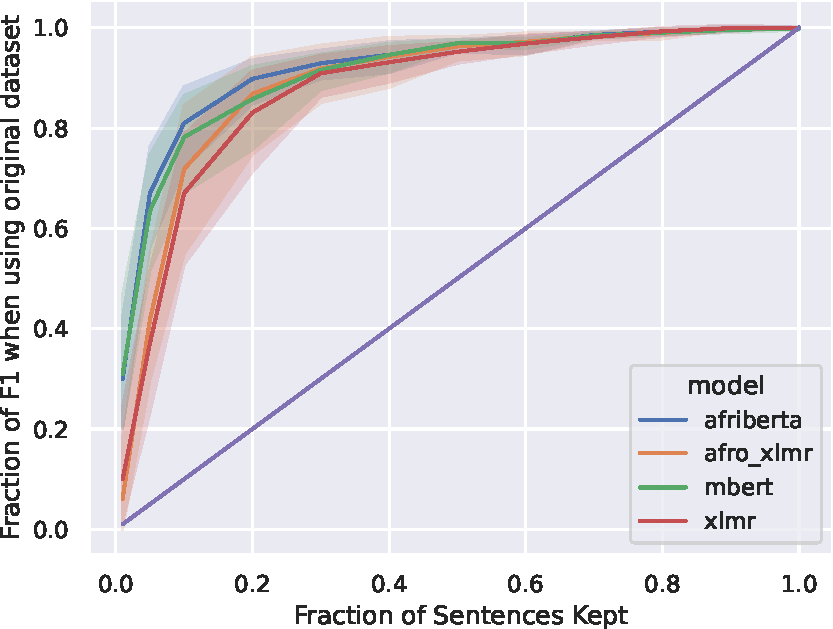
\includegraphics[width=1\linewidth]{images/global_cap_sentences.pdf}
%     \caption{Plotting the fraction of sentences kept against performance (measured as a fraction of ``optimal'' performance -- where the entire dataset is used). Standard Deviation across 11 languages is shaded.}
%     \label{fig:global_cap_sentences}
% \end{figure}

% \begin{figure}
%     \centering
%     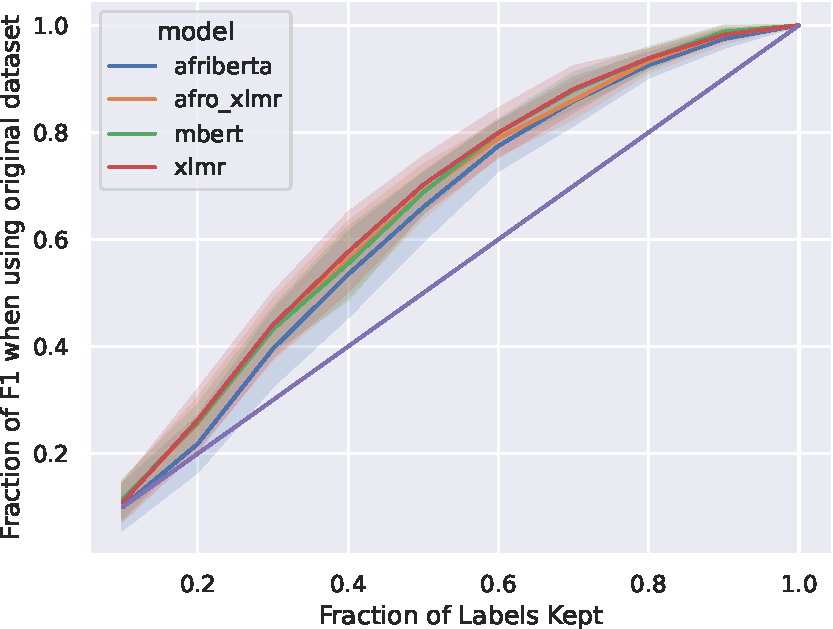
\includegraphics[width=1\linewidth]{images/global_cap_labels.pdf}
%     \caption{Deleting Labels (replacing with O)}
%     \label{fig:global_cap_labels}
% \end{figure}

% \begin{figure}
%     \centering
%     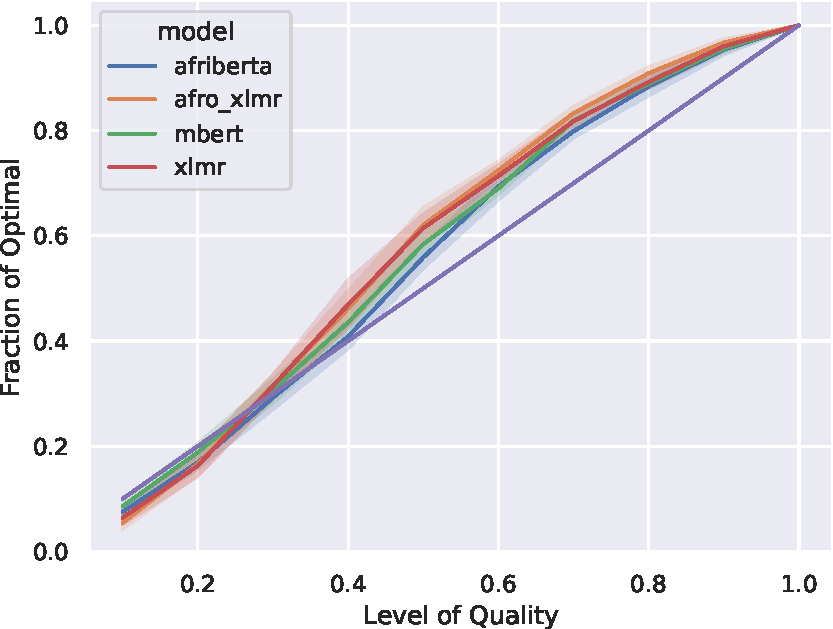
\includegraphics[width=1\linewidth]{images/global_swap_labels.pdf}
%     \caption{Swapping Labels with other entities}
%     \label{fig:global_swap_labels}
% \end{figure}



% \begin{figure}
%     \centering
%     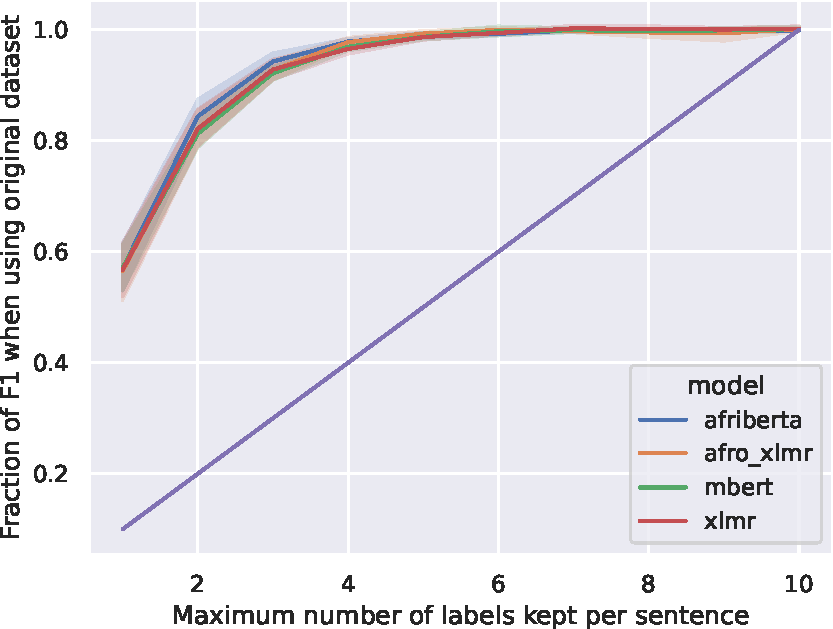
\includegraphics[width=1\linewidth]{images/local_cap_labels.pdf}
%     \caption{Local Cap Labels}
%     \label{fig:local_cap_labels}
% \end{figure}

% \begin{figure}
%     \centering
%     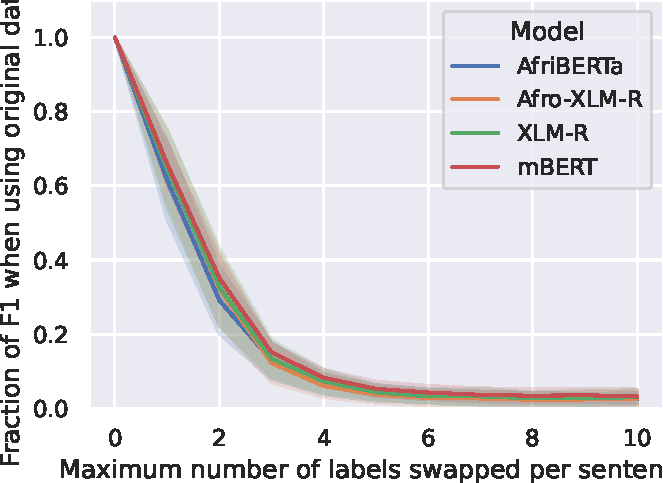
\includegraphics[width=1\linewidth]{images/local_swap_labels.pdf}
%     \caption{Local Swap Labels}
%     \label{fig:local_swap_labels}
% \end{figure}


% \begin{table}[]
%     \centering
%     \caption{Number of entities per language, broken down by type. \mike{TODO make this a bar chart? Also have more data analysis tables/figures}}
%     \label{tab:num_entities}
%     \begin{tabular}{lrrrrr}
\toprule
{} &     LOC &      ORG &    DATE &      PER &    Total \\
\midrule
amh &  1506.0 &    662.0 &   944.0 &    883.0 &   3995.0 \\
en  &  8297.0 &  10025.0 &     NaN &  11128.0 &  29450.0 \\
hau &  2379.0 &   1124.0 &  1683.0 &   1650.0 &   6836.0 \\
ibo &  1365.0 &   1167.0 &  1077.0 &   1685.0 &   5294.0 \\
kin &  2030.0 &   1209.0 &  1212.0 &   1653.0 &   6104.0 \\
lug &   829.0 &   1152.0 &   959.0 &   2099.0 &   5039.0 \\
luo &  1023.0 &    615.0 &   478.0 &    588.0 &   2704.0 \\
pcm &  1256.0 &   1329.0 &  1737.0 &   3070.0 &   7392.0 \\
swa &  2656.0 &   1522.0 &  1085.0 &   1898.0 &   7161.0 \\
wol &   587.0 &    308.0 &   300.0 &    962.0 &   2157.0 \\
yor &  1557.0 &   1327.0 &  2280.0 &   1160.0 &   6324.0 \\
\bottomrule
\end{tabular}

% \end{table}

\subsection{Entropy}
In this section we consider the effects of our data corruptions on the entropy of the models. When we progressively delete more sentences in \autoref{fig:entropy:global_cap_sentences}, the entropy steadily increases. In \autoref{fig:entropy:global_cap_labels}, we see that when we delete labels randomly, the entropy increases, reaches its peak around keeping 70\% of the labels, and then decreases again. When swapping labels, in \autoref{fig:entropy:global_swap_labels}, increasing the fraction of swapped labels decreases the entropy.

\begin{figure*}
    \centering
    \begin{minipage}[t]{0.33\linewidth}
        \captionsetup{width=.8\linewidth}
        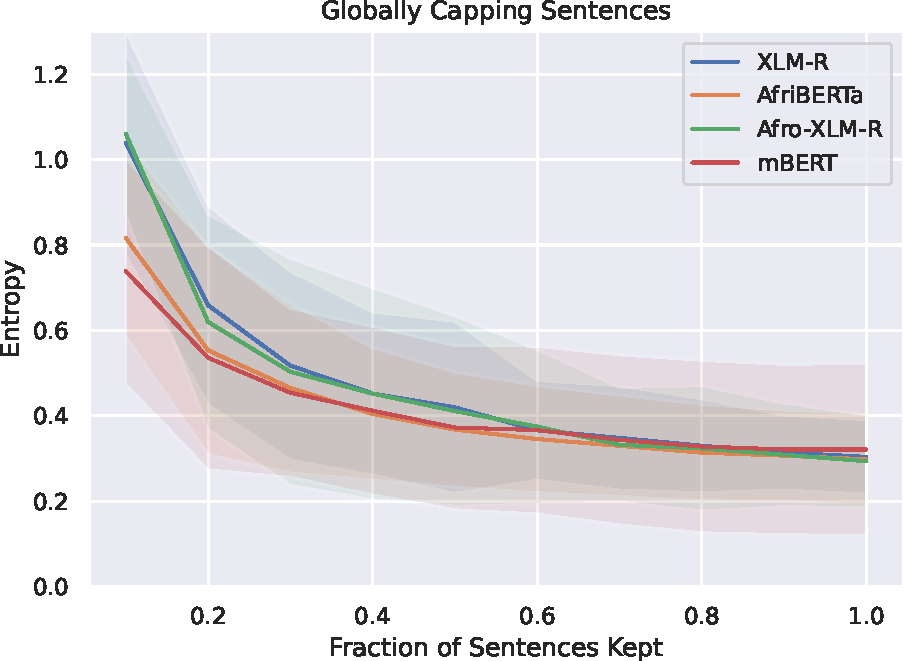
\includegraphics[width=1\linewidth]{images/ALL_global_cap_sentences.pdf}
        \caption{Showing the effect of training on a subset of data on the final performance of the models.}
        % Plotting the fraction of sentences kept against performance (measured as a fraction of ``optimal'' performance -- where the entire dataset is used). Standard Deviation across 11 languages is shaded.
        \label{fig:entropy:global_cap_sentences}
    \end{minipage}
    \begin{minipage}[t]{0.33\linewidth}
    \captionsetup{width=.8\linewidth}
        \centering
        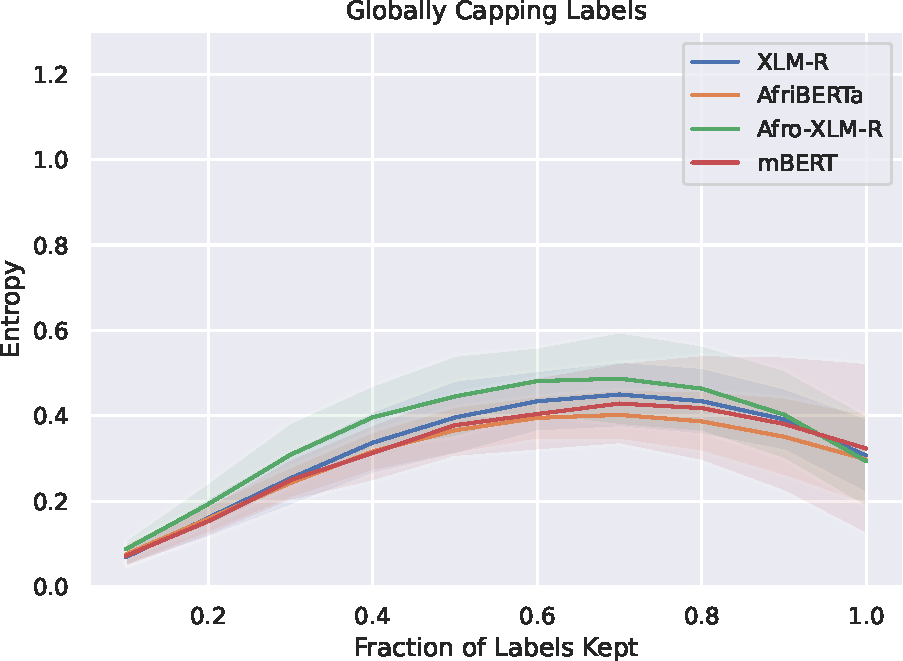
\includegraphics[width=1\linewidth]{images/ALL_global_cap_labels.pdf}
        \caption{Showing the effect of deleting a certain fraction of labels across the entire dataset, replacing them with O.}
        \label{fig:entropy:global_cap_labels}
    \end{minipage}
    \begin{minipage}[t]{0.33\linewidth}
        \captionsetup{width=.8\linewidth}
        \centering
        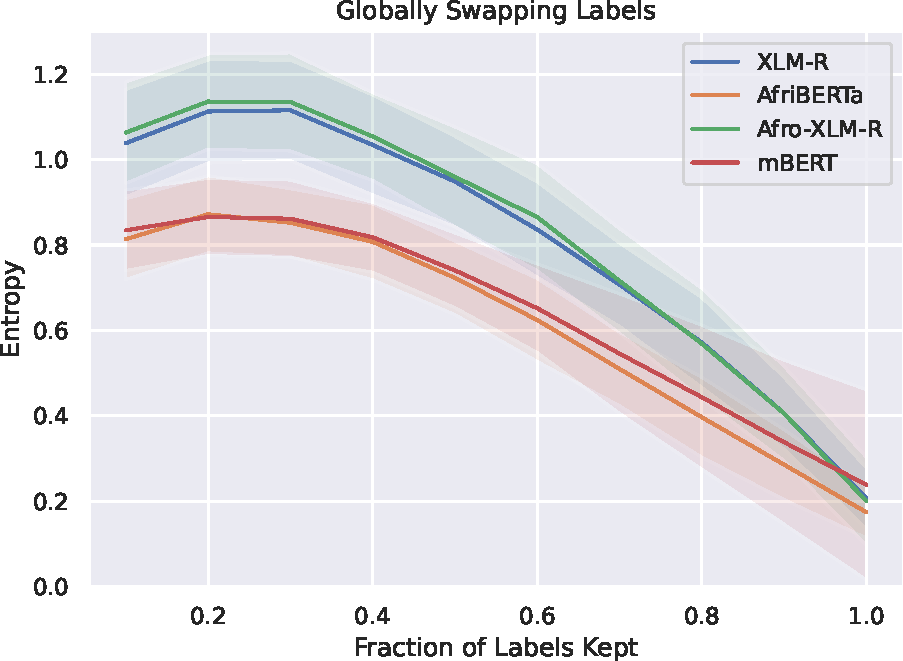
\includegraphics[width=1\linewidth]{images/ALL_global_swap_labels.pdf}
        \caption{Showing the effect of swapping a certain fraction of labels across the entire dataset, replacing the correct annotation with an incorrect entity.}
        \label{fig:entropy:global_swap_labels}
    \end{minipage}
    \caption*{Here we show the effect of each data corruption strategy on the token entropy of the models.}
\end{figure*}




\section{Discussion \& Future Work}
Our results shown above are interesting, and highlight quite a few important points. First of all, in most cases, all models exhibit roughly equal behaviour, in terms of the percentage dropoff in performance as the level of corruption increases. This ranges from the Africa-centric models (\afriberta and \afroxlmr) to the predominantly high-resourced models (XLMR and mBERT). This suggests that the behaviour we see here is quite general, as opposed to being particularly model-specific. The variation across languages is also remarkably low.

Secondly, we find that the quantity of data one trains on does not play a massive role in the final performance obtained; we could get around 80\% performance with 10-20\% of the sentences of the original dataset. This suggests that we do not need a lot of data to perform well, supporting prior findings~\citep{adelani2022Thousand}. This means that even modest data-collection and annotation efforts should be able to result in datasets that are large enough to obtain decent performance. Our results are consistent across both the languages contained in the pre-trained models' datasets and those that were not. 
% the case, even though not all of our models pre-trained on data from all of the languages we consider.
% languages, however, does not fully consider the case where the pre-trained language model has not been trained on the language under consideration.

Thirdly, the type of corruption can have a large effect on the final performance. For instance, merely leaving out annotations (e.g. replacing them with ``O'') can still result in high-performance; e.g. when keeping only 60\% of the labels, we still obtain 80\% performance. On the other hand, when we swap labels with incorrect ones, the relationship is much more linear. This suggests that having incorrect annotations is more harmful than having no annotations at all -- which could help inform annotator training in data collection endeavours.

Finally, we find that the density of entities can be of great importance. For instance, deleting 60\% of all sentences results in higher performance than deleting 60\% of all entity labels and keeping all of the sentences. Thus, having fewer sentences could be feasible, provided each of the sentences is completely, and accurately, annotated.
% \mike{We also find that deleting 60\% of all sentences results in higher performance than deleting 60\% of labels -- so density is important, high NER peformance is challenging to get when we have a low density, even when the approximate number of labels is the same.}

There are numerous avenues for future work. One option would be to expand our work into other NLP tasks; for example, additional token classification tasks such as parts of speech tagging, or tasks such as machine translation. Additionally, developing more corruption strategies that cover other components of quality would be promising as well. Furthermore, combining multiple different corruption strategies and investigating how robust models are to these. Finally, using our analysis, future work could develop better methods for dealing with corrupted datasets that would mitigate some of the effect of training on subpar data.
% \begin{enumerate}
%   \item No annot better than wrong one
%     \item All models perform roughly equally
%     \item Likewise, all languages perform roughly equally
%     \item Do not need a lot of data.
% \end{enumerate}
\section{Conclusion}
Our main aim in this paper is to systematically analyse the effect of data quality and quantity on the performance of pre-trained models on an NER task for low-resourced languages. We do this by designing multiple corruption strategies, and fine-tuning models on various degrees of corruption.
Overall, our results emphasise that pre-trained models can perform quite well with remarkably little data, and that missing annotations are less harmful than misleading ones. Ultimately, we hope that this analysis can help inform future NER dataset creation endeavours, or help NLP practitioners when needing to decide on a dataset.
\bibliographystyle{named}
\bibliography{ijcai22,bib2,bib3,bib4}

\end{document}

